
\documentclass[12pt,utf8]{article}
%%
% CUMUM Thesis template
% Created by Caibin Zeng, email: macbzeng@scut.edu.cn  %
% July 8, 2022
%%
% 承诺书页和编号专用页,直接在官网Word模板编辑,再转成PDF
% 本模板只涉及正文部分

%% 页面布局 %%
\usepackage{geometry}
\geometry{a4paper,left=2.5cm,right=2.5cm,top=2.5cm,bottom=2.5cm}

%% 必备宏包及说明 %%

% 显示中文
\usepackage{ctex}
% 章节题目居中且第一级编号设置为中文样式
\usepackage{sectsty}
\sectionfont{\centering}
\renewcommand\thesection{\chinese{section}、}
\renewcommand\thesubsection{\arabic{section}.\arabic{subsection}}
% 颜色宏包
\usepackage[dvipsnames]{xcolor}
\definecolor{dkgreen}{RGB}{0, 96, 50}

% 三线表宏包
\usepackage{booktabs}
\usepackage{makecell}
% 数学字体宏包
\usepackage{amsfonts}
% 超链接宏包
\usepackage{hyperref}
\hypersetup{colorlinks,
	linkcolor=black,
	anchorcolor=blue,
	pdfstartview=Fit,
	breaklinks=true}
% 数学公式宏包
\usepackage{amsmath}
% 表格宏包
\usepackage{multirow} 
% 图形宏包
\usepackage{graphicx} 
\usepackage{subcaption}	
\usepackage{float}
% 动画宏包
\usepackage[dvipdfmx]{animate}
%代码宏包
\usepackage{listings}
%国标引用,修改开源项目,修正学位论文中出现出版社不详的问题
\usepackage{gbt7714}

%修改目录
\usepackage{tocloft}




\lstset{
  frame=tb,
  aboveskip=3mm,
  belowskip=3mm,
  showstringspaces=false,
  columns=flexible,
  framerule=1pt,
  rulecolor=\color{gray!35},
  backgroundcolor=\color{gray!5},
  basicstyle={\small\ttfamily},
  numbers=none,
  numberstyle=\tiny\color{gray},
  keywordstyle=\color{blue},
  commentstyle=\color{dkgreen},
  breaklines=true,
  breakatwhitespace=true,
  tabsize=3,
}
\renewcommand {\lstlistingname}{源程序}

\begin{document}


%% 标题页

\begin{center} 
  % 标题
   \zihao{-2}\bfseries\heiti {论文标题(在原题目上加上亮点或主要工作)}
   \vspace{2ex}
   
   \zihao{3}\bfseries\heiti {摘要}
\end{center}


\textbf{基于全国大学生数学建模竞赛论文要求,旨在让华南理工大学参赛同学专注于论文的内容写作而不用浪费时间在论文的格式定制和调整上,数模团队特编写此 \LaTeX 模板,若有任意疑问和建议,请联系曾老师 macbzeng@scut.edu.cn。\color{blue}{Veni修改内容:修正原模板中的dkgreen颜色报错;修正原模板中插入代码的时候单行代码过长而无法显示;改变附录代码插入格式,改为lstinputlisting,直接输入文件名,不必再CV;改变文献引用格式,采用gbt7714-2015格式,同时修正了开源模板中的学位论文出现[出版社不详]的问题;修正目录与ref的颜色冲突。应该没有bug了吧。}}

基于XXX问题背景,本文建立XXX和XXX模型,研究XXX的机理/讨论XXX对XXX的影响关系/探索XXX,采用XXX方法(理论和数值)求解XXX模型,提出XXX指标/制定XXX策略,正面回答XXX问题/提出XXX建议。

针对问题 1:首先根据XXX条件,点明重点理想化假设,建立XXX模型;其次采用XXX求解方法,点明求解思路和算法实现的亮点;列出主要结果。(模型、方法、亮点、主要结果黑体突出,除图表可以采用彩色,文字不要用)

针对问题 2:首先根据XXX条件,点明重点理想化假设,建立XXX模型;其次采用XXX求解方法,点明求解思路和算法实现的亮点;列出主要结果。(模型、方法、亮点、主要结果黑体突出,除图表可以采用彩色,文字不要用)

针对问题 3:首先根据XXX条件,点明重点理想化假设,建立XXX模型;其次采用XXX求解方法,点明求解思路和算法实现的亮点;列出主要结果。(模型、方法、亮点、主要结果黑体突出,除图表可以采用彩色,文字不要用)

最后,评价模型和结果的合理性,再吹吹牛皮谈谈展望和潜在应用价值,若正文不满20页可添加灵敏性分析、模型的优劣性分析等。


\vspace{2ex}

\noindent{\heiti 关键词:} 628;Veni;YYDS



\newpage

%目录  国赛不需要目录,可以注释掉,其他比赛可一键生成
\begin{center}
	\tableofcontents
\end{center}
\newpage

% chap 1
\section{问题重述}

此为数学建模比赛论文的正文第一部分,需要将原问题进行整理,主要分两个子章节:问题背景和问题重述,难度几乎为零。但是需要强调:语言简洁精炼,避免冗长琐碎;
绝对不可照抄原题,不然过不了查重或加大重复率!

\subsection{问题背景}
   一般是对题目的前几段话的重述,可以变换文字的前后顺序、语句的语态,特别是务必添加1-3篇参考文献及其切题的描述 。
\subsection{问题重述}
   一般针对所提的3-4个问题逐一重述,主要点明:根据什么条件(一般条件和特定条件)、构建什么模型、解决什么问题。

% chap 2
\section{问题分析}

该部分主要体现数学建模从实际问题到抽象数学符号的思维过程,考查对问题的认知度,利用题目的信息和条件确定建模的思路,且隐约表明解决问题的雏形,但不要讲述任何结果或结论。一般是每个问题单独分析一个小章节,文字控制在4-8行。

\subsection{问题1的分析}
根据题目的信息和条件,查阅文献,说明模型构建的重点和难点,通常建模思路是否可行,需要如何调整和改进,做了什么合理的简化假设,说明拟构建模型的合理性和可行性。务必参考1-3篇文献。

\subsection{问题2的分析}
若基于问题1的模型求解,说明拟采用的求解方法和采用的原因,特别是困难和挑战是如何克服的,切记不要直接套用经典的求解方法,务必有改进和推广。若需要另外建立模型,参考问题1的分析思路,说明与前面模型的继承关系和不同之处,特别要强调后建模型的困难。

\subsection{问题3的分析}

根据每个问题,循序渐进地说明信息和条件的复杂、构建模型的难点、缺乏直接的求解方法而需要综合两个以上算法或者改进现有算法的尴尬、复杂模型的分解思路、复杂求解方法的分步思路等。


% chap 3
\section{模型假设}

常见的模型假设:
\begin{enumerate}
\item 题目明确给出的假设条件
\item 排除生活中的小概率事件(例如黑天鹅事件、非正常情况)
\item 仅考虑问题中的核心因素,不考虑次要因素的影响
\item 使用的模型中要求的假设
\item 对模型中的参数形式(或者分布)进行假设
\item 和题目联系很紧密的一些假设,主要是为了简化模型
\end{enumerate}

% chap 4
\section{符号说明}

本部分是对模型中使用的重要变量进行说明,一般排版时要放到一张表格中,且建议使用三线表,后面具体讲三线表,同时表格尽可能不要添加竖线。

注意:
\begin{itemize}
\item 不需要把所有变量都放到这个表里面,模型中用到的临时变量可以不放。
\item 下文中首次出现这些变量时也要进行解释,不然会降低文章的可读性。
\item \href{https://www.latexlive.com/}{\LaTeX 公式线上编辑器}
\item \href{https://www.caam.rice.edu/~heinken/latex/symbols.pdf}{\LaTeX 数学符号 (M. Heinkenschloss 教授收集) }
\end{itemize}

\begin{table}[h]
\centering
\begin{tabular}{p{2cm}<{\centering}p{9cm}<{\centering}p{2cm}<{\centering}}
   \toprule
   符号 & 说明 & 单位 \\
   \midrule
   $\alpha$ & 建模花费时间  & 天   \\
   $\mathbb{E}[X]$ & 股票收盘价$X$的数学期望 & 元 \\
   $W_{\text{max}}$ & 某人体重$W$的最大值 & 千克  \\
   $x_{ij}$ & 第$i$辆货车运输第$j$种货物的单位费用&  元/吨 \\
   \bottomrule
\end{tabular}
\end{table}

Tips: 数学符号可以参考 M. Heinkenschloss 教授收集,兼顾变量本身的实际意义,若有约定俗成的、专门的数学记号,尽量遵守通用符号,例如上表中的期望记号 $\mathbb{E}$;若自由发挥时,可以根据字面意思对应的英文的前3-4字母,例如上表的 $W_{\text{max}}$;避免出现含糊不清或歧义的符号,比如上表的 $\alpha$,可改成 $T_{\text{tol}}$;关键决策变量可以直接采用26个字母相关。总之,记号兼顾简洁和内涵。


% chap 5
\section{模型的建立与求解}

针对每个问题,逐一构建模型和求解。

\subsection{问题1模型的建立与求解}
\subsubsection{模型的建立}
首先注意模型的构建基于前面的问题问题和模型假设,大多数数学建模比赛的模型都是基于经典的成熟模型,但切忌随意套用模型,一定要有机结合题目的信息和条件,对已有模型的某一方面进行改进或者优化,(若为天之骄子可建立原创性模型),独辟蹊径(改进时切莫择易避难,应当有点难度和广度),但务必明确给出模型,这是论文的重要组成部分,同时更是创新点和亮点。
\subsubsection{模型的求解}
说明采用的求解方法,若为成熟算法应蜻蜓点水般一语带过,不要长篇大论介绍算法的背景、原理、步骤;若求解方法需要改进或有亮点的地方务必强调,但也不需要太多理论介绍;若为现代智能优化算法(如遗传算法、粒子群算法、蚁群算法、模拟退火算法、神经网络算法)或者专业软件和平台,需要阐明算法的计算步骤或算法流程图,算法的调参不需要说明,编入附录代码就行。

简明扼要地陈述求解的结果,应该遵守图表规范,并且醒目突出,若求解结果过长,建议编入附录,同时不要对结果的优劣性和合理性进行主观评述。

\subsection{问题2模型的建立与求解}

\subsubsection{模型的建立}

一般是基于问题1的模型进行深入建模或改进,一定要记得自变量和因变量都是相对的,故后续模型通常是问题1模型的反问题或者推广。切记,模型一定要明确写出。


\subsubsection{模型的求解}

一般是基于问题1的结果,若继续采用问题1的求解方法可一笔带过,若需要额外求解方法,请简要阐明计算步骤或算法流程图。

所得结果同样简洁规范,并且醒目突出,若求解结果过长,建议编入附录,同时不要对结果的优劣性和合理性进行主观评述。

\subsection{问题3模型的建立与求解}

\subsubsection{模型的建立}
在模型的建立部分,会遇到若干类型的数学公式,下面列举其中常见情形:

\begin{equation}\label{eq1}
  i\hbar\frac{\partial}{\partial t} \Psi(r,t)  = \left[
  -\frac{\hbar^2}{2m}\nabla^2+V(r,t) \right]\Psi(r,t) 
\end{equation}

\begin{equation*}
  e=\lim_{n\to\infty} \left(1+\frac{1}{n}\right)^n
\end{equation*}

\begin{equation}
   E = mc^2  \tag{MEE}
\end{equation}

%\begin{equation}
%  \left(1+x\right)ˆn  =  1 + nx + \frac{n\left(n-1\right)}{2!}x^2 
%   + \frac{n\left(n-1\right)\left(n-2\right)}{3!}x^3 
%   + \frac{n\left(n-1\right)\left(n-2\right)\left(n-3\right)}{4!}x^4 
%  +  \frac{n\left(n-1\right)\left(n-2\right)\left(n-3\right)\left(n-4\right)}{5!}x^5 \ldots
%\end{equation}

\begin{equation}
\begin{aligned}
   \left(1+x\right)ˆn  =&  1 + nx + \frac{n\left(n-1\right)}{2!}x^2 
     + \frac{n\left(n-1\right)\left(n-2\right)}{3!}x^3 
     \\& + \frac{n\left(n-1\right)\left(n-2\right)\left(n-3\right)}{4!}x^4 
   +  \frac{n\left(n-1\right)\left(n-2\right)\left(n-3\right)\left(n-4\right)}{5!}x^5 \ldots
\end{aligned}
\end{equation}

\begin{equation}
\left\{
\begin{aligned}
 \dot{x}&=f(x,y,z)\\
 \dot{y}&=g(x,y,z)\\
 \dot{z}&=h(x,y,z)\\
\end{aligned}
\right.
\end{equation}

\begin{equation*}
\begin{aligned}
&\max v  \\
\text{使得} & \\
&\begin{cases}
  \frac{|u_{i+1}-u_{i}|}{0.5}<3, 1\le i\le n\\
  60\le T_1 \le 120\\
  40 \le T_2 \le 90 \\
  240 \le u_{\text{max}} \le 250
\end{cases}
\end{aligned}
\end{equation*}

\[
\begin{pmatrix}
1 & 2 \\
3 & 4
\end{pmatrix}
\]

\[
 \begin{bmatrix}
   a_{1,1} & a_{1,2} & \cdots & a_{1,n} \\
   a_{2,1} & a_{2,2} & \cdots & a_{2,n} \\
   \vdots  & \vdots  & \ddots & \vdots  \\
   a_{n,1} & a_{n,2} & \cdots & a_{n,n} 
 \end{bmatrix}
\]

\[
\begin{cases}
 -2, & \text{if~} x\le-2 \\
 x, & \text{if~}  -2<x\le-1 \\
 2,  & \text{if~}  x\ge2 \\
\end{cases}
\]


\subsubsection{模型的求解}

模型求解会遇到算法步骤的攥写,示例如下:

\begin{description}
\item[第1步:] 数据预处理/参数设定
\item[第2步:] 应用XXX离散格式/函数来计算XXX
\item[第3步:] 利用XXX方法可得XXX
\end{description}

\begin{table}[htb]%表示放置当前位置
\caption{XXX班级个人信息汇总}
\label{tab1}%交叉引用
\begin{center}
\begin{tabular}{cccccc}
   \toprule
   序号 & 姓名 & 性别 & 年龄 & 身高/cm & 体重/kg \\
   \midrule
   1 & 张三 & M & 16 & 163 & 50 \\
   2 & 王红 & F & 15 & 159 & 47 \\
   3 & 李二 & M & 17 & 165 & 52 \\
   \bottomrule
\end{tabular}
\end{center}
\end{table}

 

\begin{table}[htb]%表示放置当前位置
\caption{XXX班级个人信息汇总}
\label{tab2}%交叉引用
\begin{center}
\begin{tabular}{*{6}{p{2cm}<{\centering}}}
   \toprule[0.1cm]
   序号 & 姓名 & 性别 & 年龄 & 身高/cm & 体重/kg \\
   \midrule[0.05cm]
   1 & 张三 & M & 16 & 163 & 50 \\
   2 & 王红 & F & 15 & 159 & 47 \\
   3 & 李二 & M & 17 & 165 & 52 \\
   \bottomrule[0.1cm]
\end{tabular}
\end{center}
\end{table}

\begin{table}[H]%表示放置当前位置
\caption{XXX社区水果和蔬菜购买汇总}
\label{tab3}%交叉引用
\begin{center}
\begin{tabular}{*{6}{p{2cm}<{\centering}}}
  \toprule
  \multirow{2}*{姓名} & \multicolumn{2}{c}{水果} & \multicolumn{2}{c}{蔬菜} & \\
  \cmidrule(lr){2-3}\cmidrule(lr){4-5}\cmidrule(lr){6-6}\morecmidrules\cmidrule(lr){6-6}
  & 苹果 & 橘子 & 白菜 & 土豆 & 共计 \\
  \midrule
  小明 & 2kg & 1kg & 1.5kg & 2kg & 6.5kg \\
  \bottomrule
\end{tabular}
\end{center}
\end{table}

如果对表格的布局不熟悉,可采用在线生成表格,链接如下:
\begin{center}
\href{https://www.tablesgenerator.com/}{Table Generator} \qquad
\href{https://tableconvert.com/}{Table Convert} \qquad
\href{https://www.latex-tables.com/}{\LaTeX Table}
\end{center}



\begin{figure}[htb]
\centering

\includegraphics[width=1\linewidth]{./figures/logo}
\caption{华南理工大学校徽、校名与数学数学院徽}
\label{fig:logo}
\end{figure}

\begin{figure}[H]
\centering
\begin{subfigure}{0.4\textwidth}
    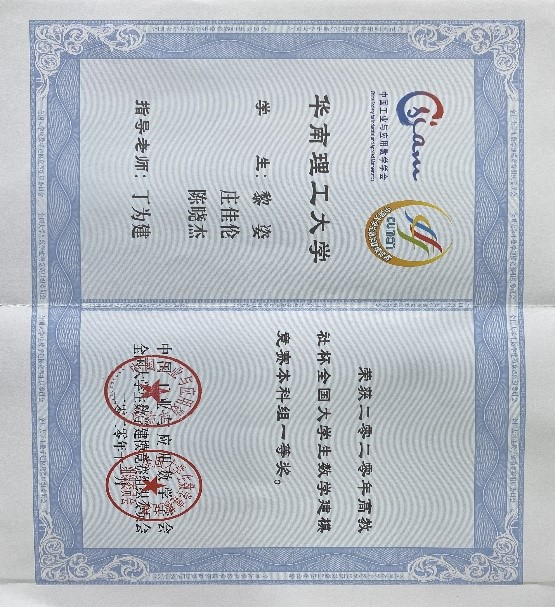
\includegraphics[width=\textwidth,angle=90]{./figures/CUMCM2020}
    \caption{2020 国赛国家一等奖}
    \label{fig:first}
\end{subfigure}
\hfill
\begin{subfigure}{0.4\textwidth}
    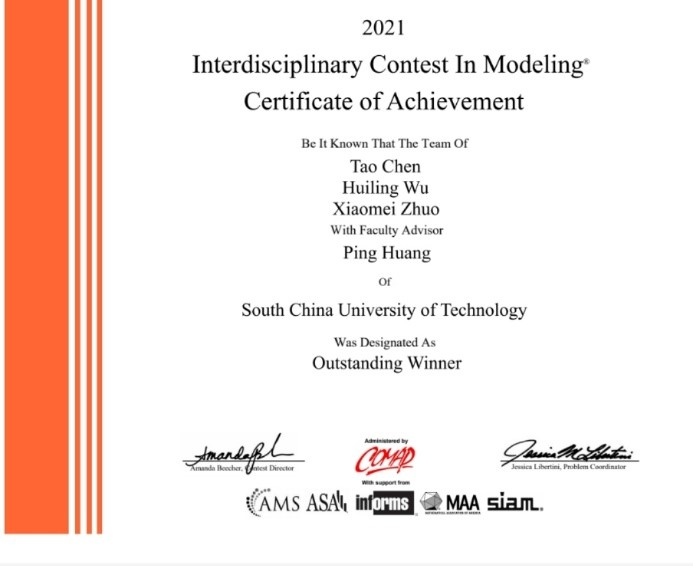
\includegraphics[width=1.2\textwidth]{./figures/MCM2021}
    \caption{2021 美赛O奖}
    \label{fig:second}
\end{subfigure}
\hfill
\begin{subfigure}{0.9\textwidth}
    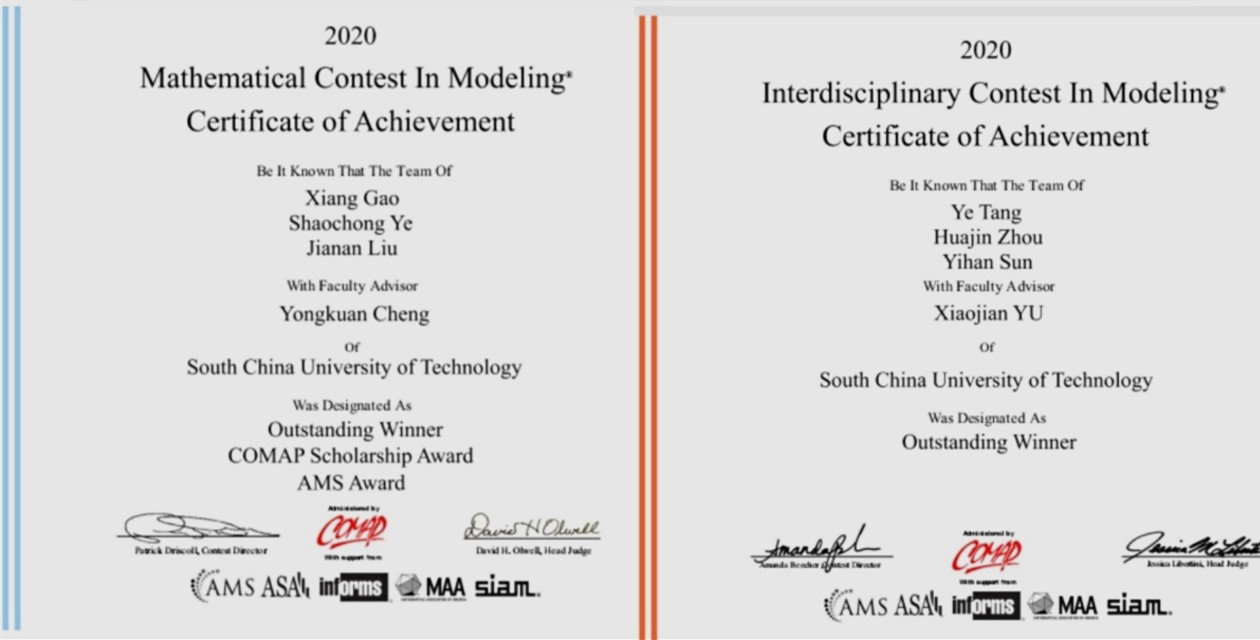
\includegraphics[width=\textwidth]{./figures/MCM2020}
    \caption{2020 美赛O奖}
    \label{fig:third}
\end{subfigure}
        
\caption{华工近两年的部分数模奖项展示}
\label{fig:figures}

\end{figure}


图表可以交互引用,但是标签(label)务必放在标题(caption)之后才能正确引用,上面提供了三线表的制作,例如表 \ref{tab1}、表 \ref{tab2}、表 \ref{tab3};对于图形,如果是单个图形,居中放置即可,如图 \ref{fig:logo},若多个子图可根据数量进行布局,可给每个子图单独赋予子标题,如图 \ref{fig:second} 所示,同时整体有个大标题,如图 \ref{fig:figures} 所示。

图像主要作用是为了直观明确地表现所得结果,可以是软件包括 MatLab、Python、C 等高级语言软件,各有千秋,故选用何种语言取决于同学们的熟练程度,掌握其一即可,推荐使用 MatLab 语言。

首先,在官网注册地址:
\href{https://ww2.mathworks.cn/mwaccount/register}{https://ww2.mathworks.cn/mwaccount/register} 采用常用邮箱注册并验证;其次,关联许可证:
     \begin{enumerate}
     \item 许可证号: 41049590,    
     激活密钥: 18066-68130-27388-35312-64164
     \item 许可证号: 41043477,    
          激活密钥: 87700-62644-49623-04064-28497
     \end{enumerate}   
然后下载matalb2022a版本并安装,约耗时20分钟。

关于图形美化,推荐使用 PlotPub 工具箱,下载地址为\href{https://www.mathworks.com/matlabcentral/fileexchange/47921-plotpub-publication-quality-graphs-in-matlab}{MatLab File Exchange} 或 \href{https://github.com/masumhabib/PlotPub}{GitHub},注意 MatLab File Exchange 包含许多MatLab开源代码,下载时需使用刚才注册的账号。下载后,解压到命名为PlotPub的文件夹,然后打开MatLab软件$ \rightarrow $ 设置路径$ \rightarrow $ 添加并包含子文件夹$ \rightarrow $选定文件夹PlotPub $\rightarrow $保存。


\begin{figure}[hb]
\centering
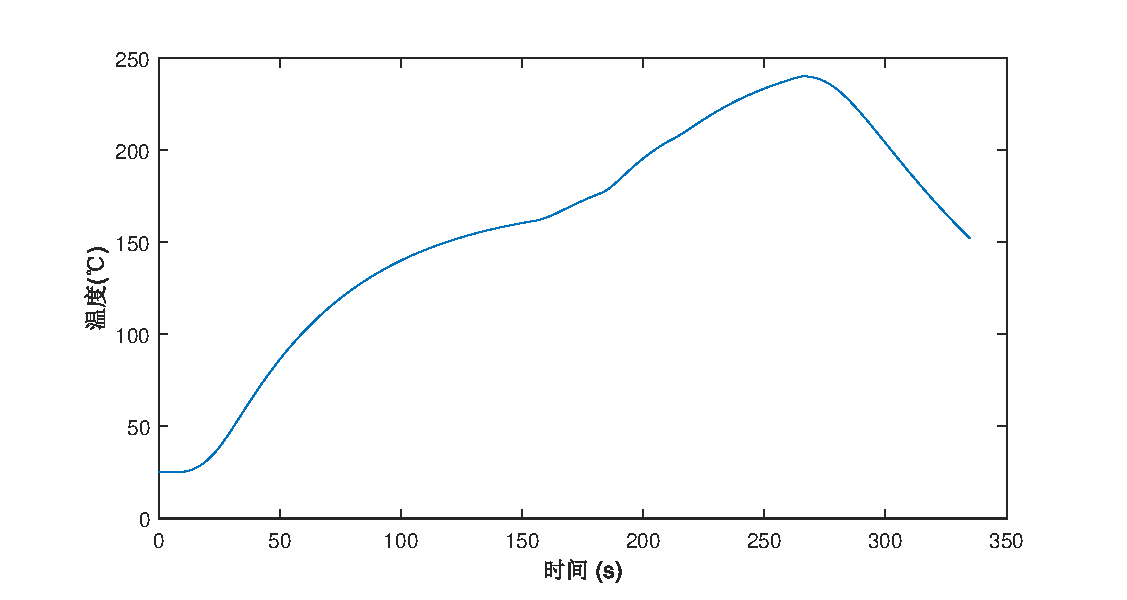
\includegraphics[width=0.85\linewidth]{./figures/OrigFig}
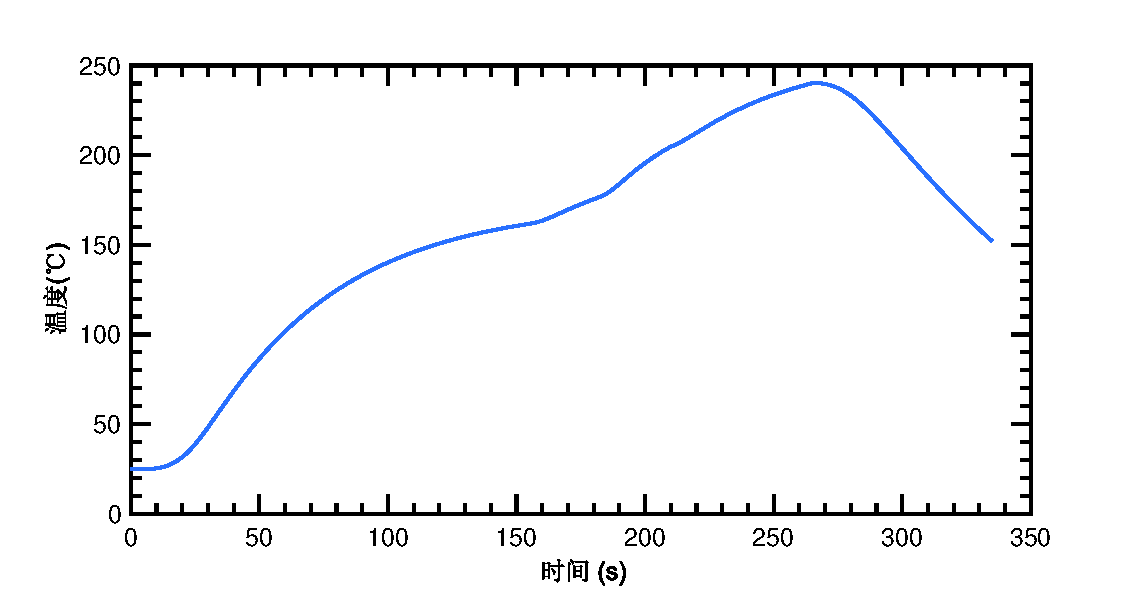
\includegraphics[width=0.85\linewidth]{./figures/BiuFig}
\caption{炉温曲线美化前后对比}
\label{fig:origfig}
\end{figure}

在图 \ref{fig:origfig} 中,只需在运行原图的 MatLab 代码的画图部分增添一句命令 Plot(~),注意此为大写的 P,坐标轴字体改成华文楷体即可。

另外,保存图形结果的方法:文件 $ \rightarrow $ 另存为 $ \rightarrow $ 保存类型旋转 eps 格式,不要保存为 png、jpg、bmp、tiff等格式(容易失真,且有时会超出页面),也不要保存为 pdf 格式(需要手动删除空白或设置保存选项,且有时会超出页面)。

为了结果的丰富性,任何动态变化的曲线都可以制作为动画,以炉温曲线为例,已经计算到时间分量 $t$ 和 温度分量 $u$,且坐标轴的范围为 $x\in[0, 350]$,$y\in[0, 250]$,对应代码如下:

\begin{lstlisting}[language=matlab]
figure;
h = plot(t(1),u(1),'-m','LineWidth',2);
set(gcf,'Position',[100 100 600 300])
set(gca,'TickLength',[0.02 0.02],'XColor',[0 0 0],'XMinorTick','on',...
    'YColor',[0 0 0],'YMinorTick','on','ZColor',[0 0 0],'ZMinorTick','on');
xlabel('时间 (s)','FontSize',12,'FontName','华文楷体');
ylabel('温度(℃)','FontSize',12,'FontName','华文楷体');
xlim([0 350]);  ylim([0 250])
Y1 = t(:); Y2 = u(:);
for m = 2:numel(Y1)
    set(h,'xData',Y1(1:m),'yData',Y2(1:m));
    drawnow;
end
\end{lstlisting}

\begin{center}
\animategraphics[width=.9\linewidth, autoplay, loop, 					controls]{24}{./AnimationDemo/AnimationDemo-}{0000}{0670}
\end{center}

关于制图,分享若干相关软件:

\href{https://www.cleverpdf.com/cn/gif-to-png}{GIF-to-PNG 线上转换器}
\qquad 
\href{https://www.geogebra.org/geometry}{几何画板 GeoGebra}
\qquad
\href{https://github.com/jgraph/drawio-desktop/releases}{流程图制作 draw.io}

\href{https://www.pexels.com/zh-cn/}{素材网 Pexels}
\qquad



% chap 6
\section{模型的检验与误差分析/灵敏度分析}

此部分根据正文篇幅而精简,确保正文尽量不超过20页。

\subsection{模型的检验}

针对每个问题的求解结果,呼应题目的限制条件,说明结果的正确性和合理性、求解算法的优越性和合理性。

\subsection{误差分析/灵敏度分析}

误差分析,考查模型中的误差来源,或者估算模型中存在的误差,一般用于预测问题或者数值计算类问题。

灵敏度分析,考查模型结果在系统参数或条件变化的敏感度,通用的步骤:控制其他参数不变的情况下,改变模型中某个重要参数的值,然后观察模型的结果的变化情况。



% chap 7
\section{模型的评价与推广}

此部分为论文的加分项,必不可少。

\subsection{模型的评价}

\subsubsection{模型的优点}
\begin{enumerate}
\item 模型针对性强,刚好描述了题目的相关要求、具有普适性,可应用到其他类型的实际问题;
\item 算法形式简洁有效、计算快速效率高、改进已有算法的某些部分。
\item 切忌加入主观评价,要客观地吹捧。
\end{enumerate}

\subsubsection{模型的缺点}

\begin{enumerate}
\item 表明迫于模型的复杂度做了一些理想化的简化的歉意,但强调不影响分析,结果接近一致;
\item 表明迫于计算代价而丢弃了某些次要条件或要求的悔意,字里行间流露出放手亦是成全的情感。
\item 但从数目上,缺点要比优点少。
\end{enumerate}

\subsection{模型的推广}
 针对上述缺点,提出完善简化处理、添加丢弃条件的可能性;模型和结果应用到解决实际问题的可行性。
 \cite{詹志辉CoevolutionaryParticleSwarmOptimizationWithBottleneckObjectiveLearningStrategyforMany-ObjectiveOptimization}
 \cite{冯茜基于改进粒子群算法的多目标优化及其应用}
 
 
% chap 8
\newpage

\bibliography{./cumcmthesisscut.bib} %调出LaTeX生成参考文献列表

Tips:参考文献必不可少,同时要注明正文具体引用位置,最好对所参考文献有一句话进行叙述与本文的关联性。参考文献如果来自不同出处,务必下载所引用的文献的原文,不要照搬别人的,因为很容易出现跟风错的现象,另外统一规范文字、记号、页码等。

\clearpage

% chap 9
\section*{附录}

\appendix

\section{支撑材料列表}
\begin{table}[htbp]
	\centering
	\begin{tabular}{cc}
		\toprule[1.5pt]
		文件名   & 功能描述 \\
		\midrule
		Data.mat & 附件数据 \\
		getTs.m & 获取空气温度分布向量 \\
		getTt.m & 获取炉温曲线向量 \\
		find\_alpha\_beta\_ga.m & 寻找最佳参数值 \\
		problem1.m & 问题1求解 \\
		problem2.m & 问题2求解 \\
		problem3.m & 问题3求解 \\
		problem4.m & 问题4求解 \\
		condition.m & 根据温度向量判断是否满足制程约束 \\
		evaluateS.m & 计算面积指标 \\
		evaluateD.m & 计算对称性指标 \\
		linminxin.m & 灵敏性分析 \\
		alpha\_beta1.mat & 最佳热传导模型参数 \\
		problem3\_Data.mat & 问题3求解结果 \\
		problem4\_Data.mat & 问题4求解结果 \\
		\bottomrule[1.5pt]
	\end{tabular}%
	\label{tab:addlabel}%
\end{table}%

\section{源程序}
 
\begin{enumerate}
\item getTs.m
\lstinputlisting[language=matlab]{code/getTs.m}
\item 源程序balabala
\end{enumerate}

\end{document}